% !TeX root = ../main.tex

\section{Seat Planning with Stochastic Demand}
    \frame{\sectionpage}

    \begin{frame}{Method Flow}
      We aim to obtain a seat planning with known demand scenarios.
      \begin{itemize}
        \item Build the formulation of Scenario-based Stochastic Programming (SSP).
        \item[-] Consider the nested relation: a smaller group can take the seats planned for the larger group.
        \item Reformulate SSP to the Benders Master Problem (BMP) and subproblem.
        \item The optimal solution can be obtained by solving BMP iteratively. 
      \end{itemize}
    \end{frame}

    \begin{frame}{Scenario-based Stochastic Programming (SSP)}
      % \scriptsize
      \begin{scriptsize}
        Objective: maximize the expected number of people

        $y_{i \omega}^{+}$: excess supply for $i, \omega$. $y_{i \omega}^{-}$: shortage of supply for $i, \omega$.

        $d_{i \omega}$: demand of type $i$ groups for scenario $\omega$

      \begin{equation}
        \begin{aligned}
        \hspace{-10mm}
        \max \quad & E_{\omega}\left[\sum_{i=1}^{M-1} (n_i-\delta) (\sum_{j= 1}^{N} x_{ij} + y_{i+1,\omega}^{+} - y_{i \omega}^{+}) + (n_{M}-\delta) (\sum_{j= 1}^{N} x_{Mj} - y_{M \omega}^{+})\right] \\
        \text {s.t.} \quad & \sum_{j= 1}^{N} x_{ij}-y_{i \omega}^{+}+
        y_{i+1, \omega}^{+} + y_{i \omega}^{-}=d_{i \omega}, \quad i = 1,\ldots,M-1, \omega \in \Omega \\
        & \sum_{j= 1}^{N} x_{ij} -y_{i \omega}^{+}+y_{i \omega}^{-}=d_{i \omega}, \quad i = M, \omega \in \Omega \\
        & \sum_{i=1}^{M} n_{i} x_{ij} \leq L_j, j \in \mathcal{N}\\
        & y_{i \omega}^{+}, y_{i \omega}^{-} \in \mathbb{N}, \quad i \in \mathcal{M}, \omega \in \Omega \\
        & x_{ij} \in \mathbb{N}, \quad i \in \mathcal{M}, j \in \mathcal{N}.
        \end{aligned}
      \end{equation}
      \end{scriptsize}

      \begin{tiny}
        $E_{\omega}\left[\sum_{i=1}^{M-1} (n_i-\delta) (\sum_{j= 1}^{N} x_{ij} + y_{i+1,\omega}^{+} - y_{i \omega}^{+}) + (n_{M}-\delta) (\sum_{j= 1}^{N} x_{Mj} - y_{M \omega}^{+})\right]$ = $\sum_{j =1}^{N} \sum_{i=1}^M i \cdot x_{ij} - \sum_{\omega =1}^{|\Omega|} p_{\omega} \sum_{i = 1}^{M} y_{i \omega}^{+}$
      \end{tiny}
    \end{frame}

\begin{frame}{Reformulation}
  \begin{columns}
    \begin{column}{0.49\textwidth}
      \begin{scriptsize}
        \begin{equation*}
          \begin{aligned}
          \hspace{-10mm}
          \max \quad & \mathbf{c}^{\intercal} \mathbf{x} + \sum_{\omega \in \Omega} p_{\omega} 
          {\color{violet} \mathbf{f}^{\intercal} \mathbf{y}_{\omega}} \\
          \text {s.t.} \quad & {\color{red}\sum_{j= 1}^{N} x_{ij}-y_{i \omega}^{+}+
          y_{i+1, \omega}^{+} + y_{i \omega}^{-}=d_{i \omega}}, \\ & i = 1,\ldots,M-1, \omega \in \Omega \\
          & {\color{red}\sum_{j= 1}^{N} x_{ij} -y_{i \omega}^{+}+y_{i \omega}^{-}=d_{i \omega}}, \\ & i = M, \omega \in \Omega \\
          & {\color{green}\sum_{i=1}^{M} n_{i} x_{ij} \leq L_j}, j \in \mathcal{N}\\
          & y_{i \omega}^{+}, y_{i \omega}^{-} \in \mathbb{N}, \quad i \in \mathcal{M}, \omega \in \Omega \\
          & x_{ij} \in \mathbb{N}, \quad i \in \mathcal{M}, j \in \mathcal{N}.
          \end{aligned}
        \end{equation*}
        \end{scriptsize}
        \begin{tiny}
              $\mathbf{c}^{\intercal} \mathbf{x} =\sum_{j=1}^{N} \sum_{i=1}^{M} i x_{ij}$, 
              $\mathbf{f}^{\intercal} \mathbf{y}_{\omega} = - \sum_{i=1}^{M} y_{i \omega}^{+}$.
              % $\mathbf{V}$ is the system matrix for $\mathbf{y}$.
        \end{tiny}
    \end{column}
    \begin{column}{.02\textwidth}
      \rule{.1mm}{0.7\textheight}
  \end{column}
    \begin{column}{0.49\textwidth}
      \scriptsize
      SSP is equivalent to the following master problem
      \begin{equation}\label{BD_master}
        \begin{aligned}
      \max \quad & \mathbf{c}^{\intercal} \mathbf{x}+ z(\mathbf{x}) \\
      \text {s.t.} \quad & {\color{green}\mathbf{x}^{\intercal} \mathbf{n} \leq \mathbf{L}} \\
      & \mathbf{x} \in \mathbb{N}^{M \times N, +},
      \end{aligned}
      \end{equation}

      where $z(\mathbf{x})$ is defined as 

    $$z(\mathbf{x}) := E(z_{\omega}(\mathbf{x})) = \sum_{\omega \in \Omega} p_{\omega} z_{\omega}(\mathbf{x}),$$ and for each scenario $\omega \in \Omega$, the subproblem

\begin{equation}\label{BD_sub}
  \begin{aligned}
    z_{\omega}(\mathbf{x}) := \max \quad & {\color{violet} \mathbf{f}^{\intercal} \mathbf{y}_{\omega}} \\
    \text {s.t.} \quad & {\color{red}\mathbf{x} \mathbf{1} + \mathbf{V} \mathbf{y}_{\omega} = \mathbf{d}_{\omega}} \\
     & \mathbf{y} \geq 0.
  \end{aligned}
  \end{equation}
    \end{column}
\end{columns}
\end{frame}

% \begin{frame}{Reformulation}
%   \small
%   Problem \eqref{sto_form} is equivalent to the following master problem
%   \begin{equation}\label{BD_master}
%     \begin{aligned}
%   \max \quad & \mathbf{c}^{\intercal} \mathbf{x}+ z(\mathbf{x}) \\
%   \text {s.t.} \quad & \mathbf{n} \mathbf{x} \leq \mathbf{L} \\
%   & \mathbf{x} \in \mathbb{N}^{M \times N, +},
%   \end{aligned}
%   \end{equation}

%   where $z(\mathbf{x})$ is defined as 

% $$z(\mathbf{x}) := E(z_{\omega}(\mathbf{x})) = \sum_{\omega \in \Omega} p_{\omega} z_{\omega}(\mathbf{x}),$$ and for each scenario $\omega \in \Omega$, we have the subproblem

%   \begin{equation}\label{BD_sub}
%     \begin{aligned}
%       z_{\omega}(\mathbf{x}) := \max \quad & \mathbf{f}^{\intercal} \mathbf{y}_{\omega} \\
%       \text {s.t.} \quad & \mathbf{x} \mathbf{1} + \mathbf{V} \mathbf{y}_{\omega} = \mathbf{d}_{\omega} \\
%        & \mathbf{y} \geq 0.
%     \end{aligned}
%     \end{equation}

%     \begin{tiny}
%     $\mathbf{c}^{\intercal} \mathbf{x} =\sum_{j=1}^{N} \sum_{i=1}^{M} i x_{ij}$, $\mathbf{f}^{\intercal} \mathbf{y}_{\omega} = - \sum_{i=1}^{M} y_{i \omega}^{+}$, $\mathbf{V}$ is the system matrix for $\mathbf{y}$.
%     \end{tiny}
% \end{frame}

\begin{frame}{Solution to Subproblem}
  Problem \eqref{BD_sub} is easy to solve with a given $\mathbf{x}$ from the perspective of the dual problem:

  \begin{equation}\label{BD_sub_dual}
    \begin{aligned}
      \min \quad & \alpha^{\intercal}_{\omega} (\mathbf{d}_{\omega}- \mathbf{x} \mathbf{1}) \\
      \text {s.t.} \quad & \alpha^{\intercal}_{\omega} \mathbf{V} \geq \mathbf{f}^{\intercal}
    \end{aligned}
    \end{equation}

    \begin{itemize}
      \item The feasible region of problem \eqref{BD_sub_dual}, $P= \{\alpha|\alpha^{\intercal} \mathbf{V} \geq \mathbf{f}^{\intercal}\}$, is bounded. In addition, all the extreme points of $P$ are integral.
      \item The optimal solution can be obtained directly according to the complementary slackness property.
    \end{itemize}
\end{frame}

\begin{frame}{Benders Decomposition Procedure}
  \small
  Let $z_{\omega}$ be the lower bound of problem \eqref{BD_sub_dual}, SSP can be obtained by solving following benders master problem:
  \begin{equation}\label{BD_master2}
    \begin{aligned}
      \max \quad & \mathbf{c}^{\intercal} \mathbf{x} + \sum_{\omega \in \Omega} p_{\omega} z_{\omega} \\
      \text {s.t.} \quad & \mathbf{x}^{\intercal} \mathbf{n} \leq \mathbf{L} \\
      & (\alpha^{k})^{\intercal}(\mathbf{d}_{\omega}- \mathbf{x} \mathbf{1}) \geq z_{\omega}, \alpha^k \in \mathcal{O}, \forall \omega \\
       & \mathbf{x} \in \mathbb{N}^{M \times N, +}
    \end{aligned}
\end{equation} 

  Constraints will be generated from problem \eqref{BD_sub_dual} until an optimal solution is found.

  \begin{figure}[ht]
    \centering
    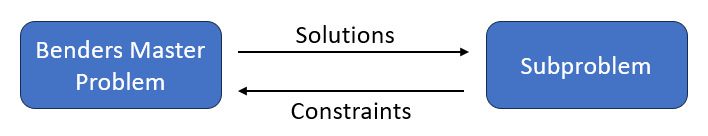
\includegraphics[width = 0.6\textwidth]{./images/BD.png}
  \end{figure}
\end{frame}


% There exists an optimal solution to SSP such that the patterns associated with this optimal solution are composed of the full or largest patterns under any given scenarios.

% \begin{frame}{Issue of Optimality}
%   \begin{itemize}
%   \item In most cases, the optimal solution can be obtained.
%   \vspace{0.5cm}
%   \item For the extreme case where the optimal solution cannot be obtained, obtaining a feasible solution did not take too much time. 
%   \vspace{0.5cm}
%   \item It is more time-consuming to verify that it is the optimal solution. Thus, we set a time limit to obtain a feasible solution.
%   \vspace{0.5cm}
%   \item 
%   \end{itemize}
% \end{frame}

\begin{frame}{Obtain Seat Planning Composed of Full or Largest Patterns}
  Challenge: it is hard to solve SSP in some cases. 
  \vspace{0.5cm}

  Property: there exists an optimal solution to SSP such that the patterns associated with this {\color{red} optimal solution} are composed of the {\color{red} full or largest patterns} under any given scenarios.
  \vspace{0.5cm}

  We aim to obtain a seat planning composed of full or largest patterns by the optimal solution to the LP relaxation of SSP.

  \begin{itemize}
    \item[-] Obtain the solution to the relaxed SSP, $\mathbf{x}^{*}$, by benders decomposition. Aggregate $\mathbf{x}^{*}$ to the number of each group type, ${s}_{i} =\sum_{j} x^{*}_{ij}, i \in \mathbf{M}$.

    \item[-] Obtain the optimal solution, $\mathbf{x}^{1}$, by solving problem \eqref{deter_upper} with $d_{i} = {s}_{i}$. 
    % Aggregate $\mathbf{x}^{1}$ to the number of each group type, ${s}_{i}^{1} = \sum_{j} x^{1}_{ij}, i \in \mathbf{M}$.
     
    \item[-] Obtain full or largest patterns by solving problem \eqref{improve_seat} with $\bm{H} = \mathbf{x}^{1}$.
 \end{itemize}
\end{frame}
